\section{数据核查与评分端点}\label{sec:data}

\subsection{数据全景与样本对应}

八个附件表可按“化学输入—感官目标—评分卡—旁证”四层归并，样本主键在 1.csv、4.csv、7.csv 与 8.xlsx 之间一致。表\ref{tab:data} 汇总了各表的规模、内容与用途：1.csv 是化学主表，4.csv 是感官监督表，2.csv、5.csv、6.csv 给出相关结构，3.xlsx 定义评分维度，7.csv 与 8.xlsx 分别提供评论旁证和外部校准。附件与公开逐人评分的数据来源见\cite{schreurs2024,zenodo2026}。

\begin{table*}[t]
\centering\small\renewcommand{\arraystretch}{1.15}
\caption{八个附件表的规模、内容与本文用途}
\label{tab:data}
\begin{tabular}{@{}>{\raggedright\arraybackslash}p{0.075\textwidth}>{\raggedright\arraybackslash}p{0.135\textwidth}>{\raggedright\arraybackslash}p{0.435\textwidth}>{\raggedright\arraybackslash}p{0.275\textwidth}@{}}
\toprule
文件 & 规模 & 内容 & 本文用途 \\
\midrule
1.csv & $250\times234$ & 3 列样本信息（beer、beer\_id、风格）+ 231 个数值字段：226 个化合物、5 个综合量 & 化学输入；风格标签与样本对齐 \\
2.csv & $231\times231$ & 231 个化学字段的秩相关矩阵（含行名列共 232 列） & 核对相关结构；构建化学网络 \\
3.xlsx & 12 卡 + 汇总 & 12 张 beer\_* 评分卡 + 1 个 summary；单卡 $100\times33$，summary $13\times52$ & 评分维度定义与目标映射 \\
4.csv & $250\times53$ & 3 列样本信息 + 50 个标准化感官目标（15 A + 15 F + 20 其他） & 目标定义与样本对应；不作 0--6 标签 \\
5.csv & $50\times51$ & 50 个感官目标间的 Spearman 矩阵 & 目标相关性核查与分组 \\
6.csv & $44\times51$ & 44 个化学字段 $\times$ 50 个感官目标的 Spearman 矩阵 & 关键因素筛选的旁证；不作因果解释 \\
7.csv & $250\times189$ & 3 列样本信息 + 186 个 Ratebeer 评论感官词 & 旁证；750 个缺失，不作训练标签 \\
8.xlsx & 7 个 sheet & 70 个校准化学字段（$250\times73$）；阈值 261 行（43 个有数值）；SHAP 500 行；MDI 232 行；价格表 & 尺度反查、第三问阈值、重要性交叉核对 \\
\bottomrule
\end{tabular}
\end{table*}

样本规模为 250 款酒、22 种风格。1.csv 的 231 个数值字段由 226 个化合物和 5 个综合量（\texttt{kcalperc}、\texttt{esters\_sum}、\texttt{aroma\_hops\_sum}、\texttt{acids\_sum}、\texttt{sulfur\_sum}）组成；4.csv 的 50 个目标由 15 个 Aroma、15 个 Flavour 和 20 个其他维度组成。1.csv 与 4.csv 均以 beer 为唯一键、beer\_id 为条码辅助键，250 行的风格标签在两表中一致，样本对应可按编号与行序双重核对，风格分层因此可直接复用，不需要另行匹配。风格样本量从 Faro 的 3 款到 Blond 的 31 款，9 种风格不足 10 款，后续按风格分层划分，避免稀有风格整体落入某一折。

\begin{figure}[t]
\centering
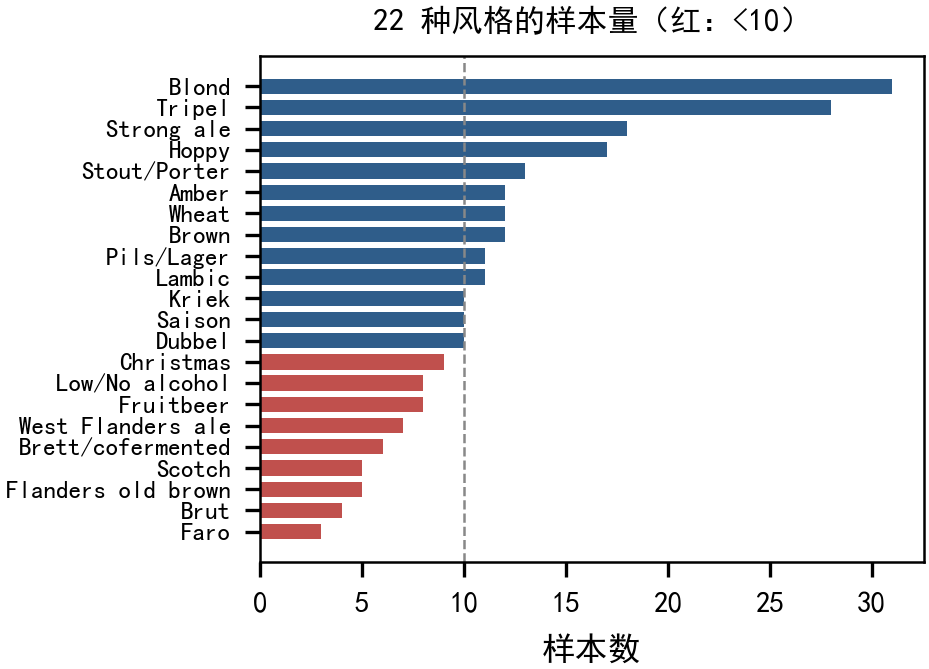
\includegraphics[width=0.95\columnwidth]{figures/fig04_styles.png}
\caption{22 种风格的样本量。红色为不足 10 款的 9 种风格，最少 3 款；分层划分与风格基线都受这一分布约束。}
\label{fig:styles}
\end{figure}5.csv 与 6.csv 分别刻画感官目标之间、化学字段与感官目标之间的秩相关结构；两表用于检查目标分块和因素筛选的方向一致性，不进入预测模型，也不进入第一问特征矩阵，避免把目标间相关当作输入信息造成泄漏。

题面与附件存在三处口径差异，本文以附件为准。题面称 226 款酒，附件为 250 款；题面称约 40 维感官目标，附件为 50 维，其中 Aroma/Flavour 各 15 项、合计 30 项；题面的约 40 维来自两栏各约 20 项的口径，附件把三组汇总和共用维度拆开后为 50 项。题面称评分卡 10 个 sheet，附件为 12 个 beer\_* 评分卡，另加 1 个 summary。四个表共用 beer 编号，使按酒划分训练折时不会出现样本错位。提交口径相应定为：50 项全部建模并输出，30 个核心项单列误差与分布指标，20 个其他项用于缺陷约束和总体评价，不与核心项合并平均。

附件 2 是秩相关矩阵，不是题面所称的皮尔逊相关矩阵。在 212 个可匹配字段上，2.csv 与本地重算 Spearman 的平均绝对差为 $1.6\times10^{-16}$，与 Pearson 的平均绝对差为 0.0883；前者处于机器精度，后者高出一个量级。因此第二问的化学网络按秩相关构建，2.csv 直接作为相关结构使用，题面的“皮尔逊”表述予以纠正。231 个字段中有 19 个因命名或汇总口径无法与 8.xlsx 的化学名匹配，核对只在 212 个可匹配字段上进行；这一限制不影响秩相关判断。8.xlsx 的 7 个 sheet 分别承载校准化学值、感官阈值、SHAP、MDI 与价格；阈值表 261 行中只有 43 行有数值，第三问的缺陷阈值只取有数值的行。

\subsection{化学尺度与异常}\label{sec:scale}

1.csv 包含经不同规则处理的化学与理化字段，不能把所有字段统一按 $10^x$ 还原。以附件 8 校准表与附件 1 中 70 个同名数值字段进行逐字段比较：对每个字段分别测试恒等、非正值替换及替换后取 $\log_{10}$ 的候选规则。38 个字段在全部可比记录上满足数值容差，其中 37 个符合“非正值替换为该字段最小正值的一半，再取 $\log_{10}$”的规则，另一个 \texttt{diethyl.succinate} 满足恒等对应；其余 32 个字段共保留 80 个不一致单元格。两组的 38 和 32 互不重叠，覆盖全部 70 个字段。

对 \texttt{diethyl.succinate}，247 个共同可比记录中，两表原值的最大绝对差为 $5.0\times10^{-10}$。该字段属于恒等对应：若把附件 1 的值误作对数并计算 $10^x/\mathrm{cal}$，比值中位数为 13.95，但各记录范围为 6.26--738.07，说明这是套用不匹配变换产生的差异，不能据此声称该字段有固定倍数的单位偏差。表间一致也不能替代独立仪器标定。

图\ref{fig:scale}(a) 展示 37 个对数规则字段的 8452 个正参考值配对；绘图仅对每个字段使用其原报告单位比较，零值替换记录不在该图中。(b) 按字段统计 80 处例外，排名前八的字段分别列出，其余24字段合并。两幅子图使用不同的数量口径，完整字段分类、变换规则和异常数见附录\ref{app:fieldsets}与支撑材料。

\begin{figure*}[t]
\centering
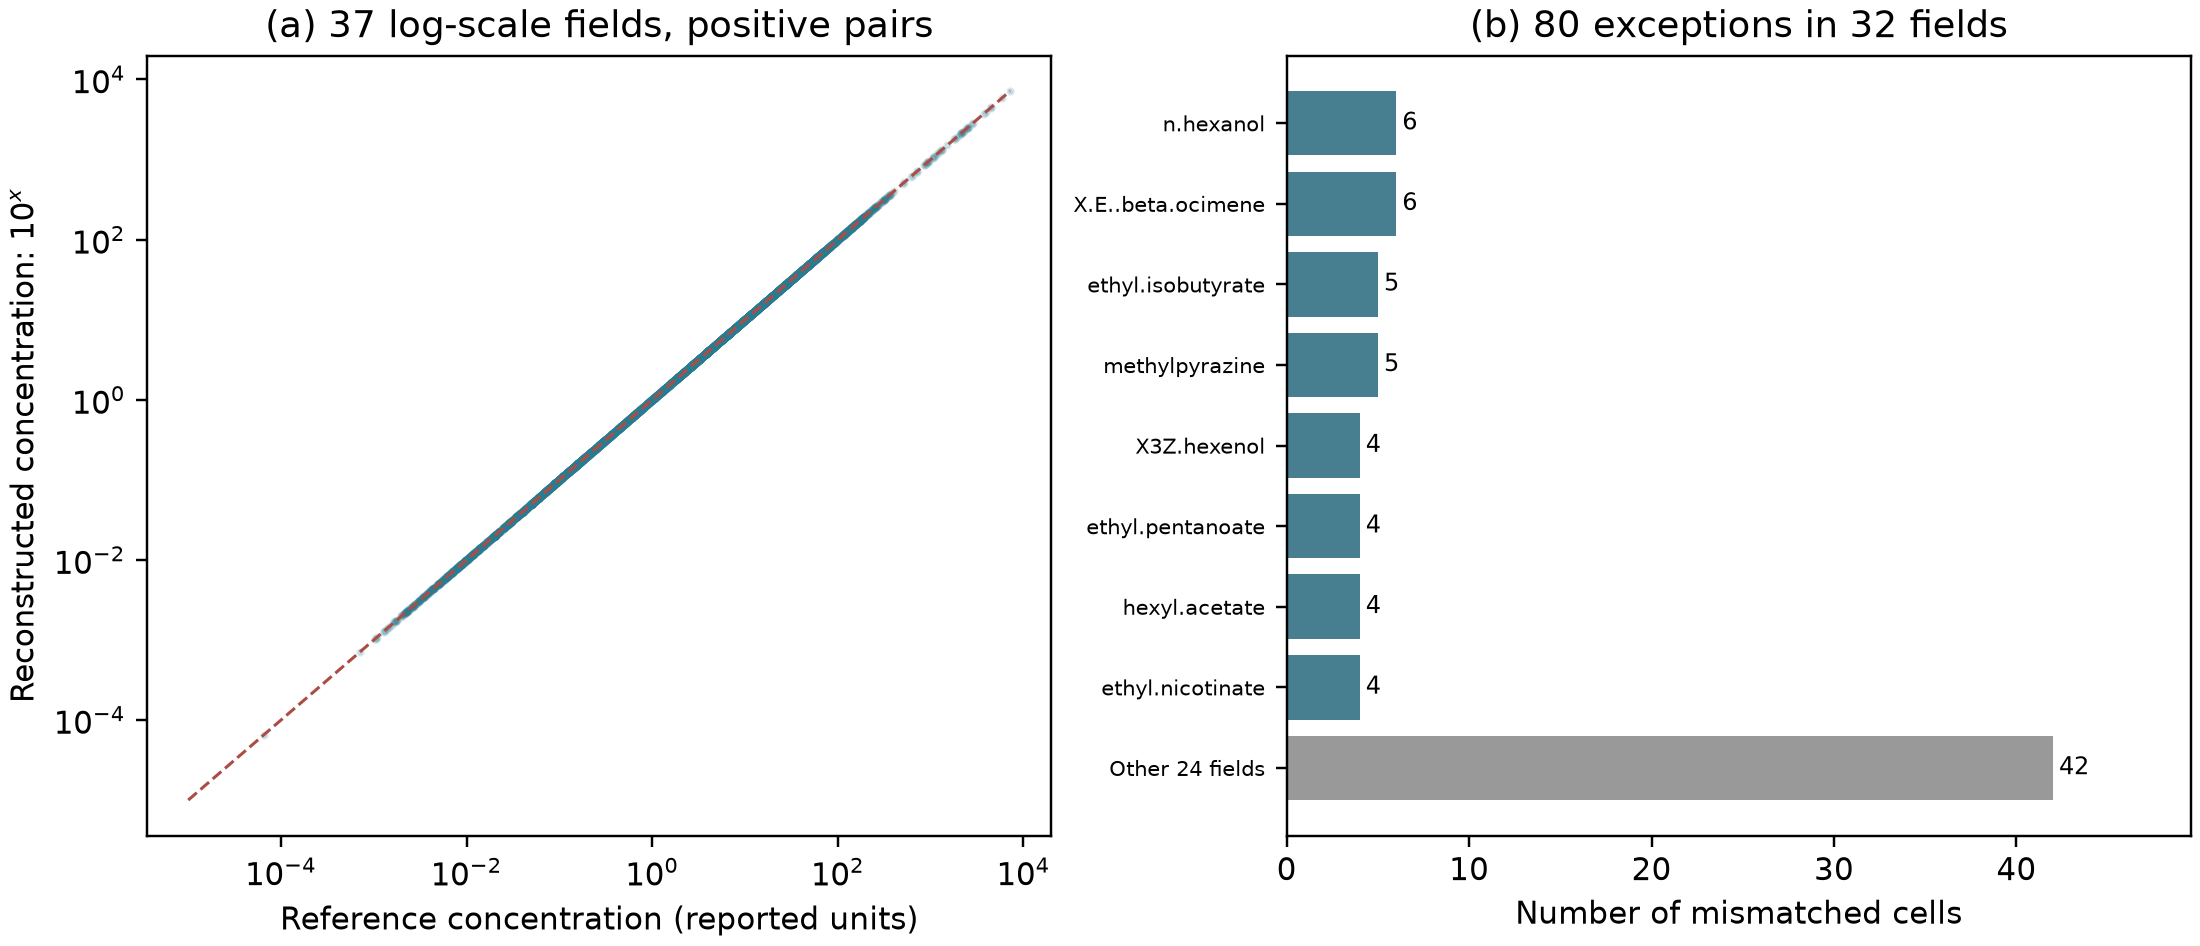
\includegraphics[width=0.98\textwidth]{figures/fig02_scale.png}
\caption{化学尺度核查。(a) 37 个对数规则字段的正值配对，各字段按自身报告单位比较；(b) 32 个不一致字段中异常单元格的数量分布，前八字段单列，其余24字段合计。}
\label{fig:scale}
\end{figure*}

第二问的另一组 32 个字段记为 $V=R\cap U\cap X_{226}$：$R$ 是上述 38 个全部可比记录一致字段，$U$ 是单位注册表中的61个字段，$X_{226}$ 是剔除5个综合量后的非综合输入。$V$ 包括31个对数规则字段和1个恒等对应字段，与80处例外所涉及的32个字段交集为空。该交集仅说明数值对应和单位记录具备，不构成完整化学标定；具体字段与单位列在附录\ref{app:fieldsets}。异常处理敏感性保留原始字段并将80处单元格置缺，填补参数只由训练折估计；另一项对照则更换为 $V$，两者回答不同问题。

\begin{table}[t]
\centering\small
\caption{化学尺度核查的集合定义}
\label{tab:scale}
\begin{tabular}{@{}p{.45\columnwidth}p{.16\columnwidth}p{.30\columnwidth}@{}}
\toprule
集合 & 字段数 & 核查结果\\
\midrule
逐点一致 $R$ & 38 & 37 对数规则、1 恒等规则\\
有例外字段 $E$ & 32 & 共80个异常单元格\\
敏感性子集 $V$ & 32 & $R\cap U\cap X_{226}$；$V\cap E=\varnothing$\\
\bottomrule
\end{tabular}
\end{table}

\subsection{缺失、低值和变换}\label{sec:missing}

显式缺失只有 73 格（0.126\%），但低值密集覆盖 18.7\% 的数值单元格，两者性质不同。73 个缺失分布在 9 列、63 款酒上，最多的一列是 \texttt{amyl.acetate} 的 27 格；9 列中 4 列的缺失不超过 2 格，\texttt{amyl.acetate} 一列接近全部缺失的 37\%。缺失列中既有建模需要的香气化合物，也有 1 个综合量 \texttt{aroma\_hops\_sum}；整列删除会改变输入维度，综合量又不能按单列均值填补，否则会破坏它与子项的关系，故按单元格保留。缺失呈点状分布，没有整行删除；本文不删除缺失行，树模型与线性模型均使用训练折估计的中位数进行填补，避免测试折信息泄漏。

数值小于 0 的单元格有 10797 个，占 18.7\%，175 个字段出现过负值。1.csv 存的是 $\log_{10}$ 浓度，负值对应原始浓度小于 1，属于低值密集而不是缺失；若按缺失删除，会丢掉近两成有效信息并系统性剔除低浓度样本。低值密集不是数据质量问题，而是浓度量级分布的直接结果，负值携带的是低浓度信息；负值占比在不同化合物间差异很大，说明低值密集不是全局缩放造成的，而是各化合物的浓度分布不同。本文保留负值，树模型直接使用，线性模型只在训练折内估计标准化参数。

7.csv 的 750 个缺失集中在 3 列，且 186 个字段来自 Ratebeer 评论词，不是品评小组的 0--6 评分。750 个缺失对应 3 个整列缺失，说明这些感官词在评论语料中没有覆盖，而不是随机漏填；评论词的出现还受文本长度和用户习惯影响，缺失机制不是随机的。因此 7.csv 只作旁证，不能作训练标签；它的 186 个评论词与 4.csv 的 50 个目标并非同一套词表，不能按名称直接合并，若用评论词训练，会把文本噪声当成感官信号。

\begin{figure*}[t]
\centering
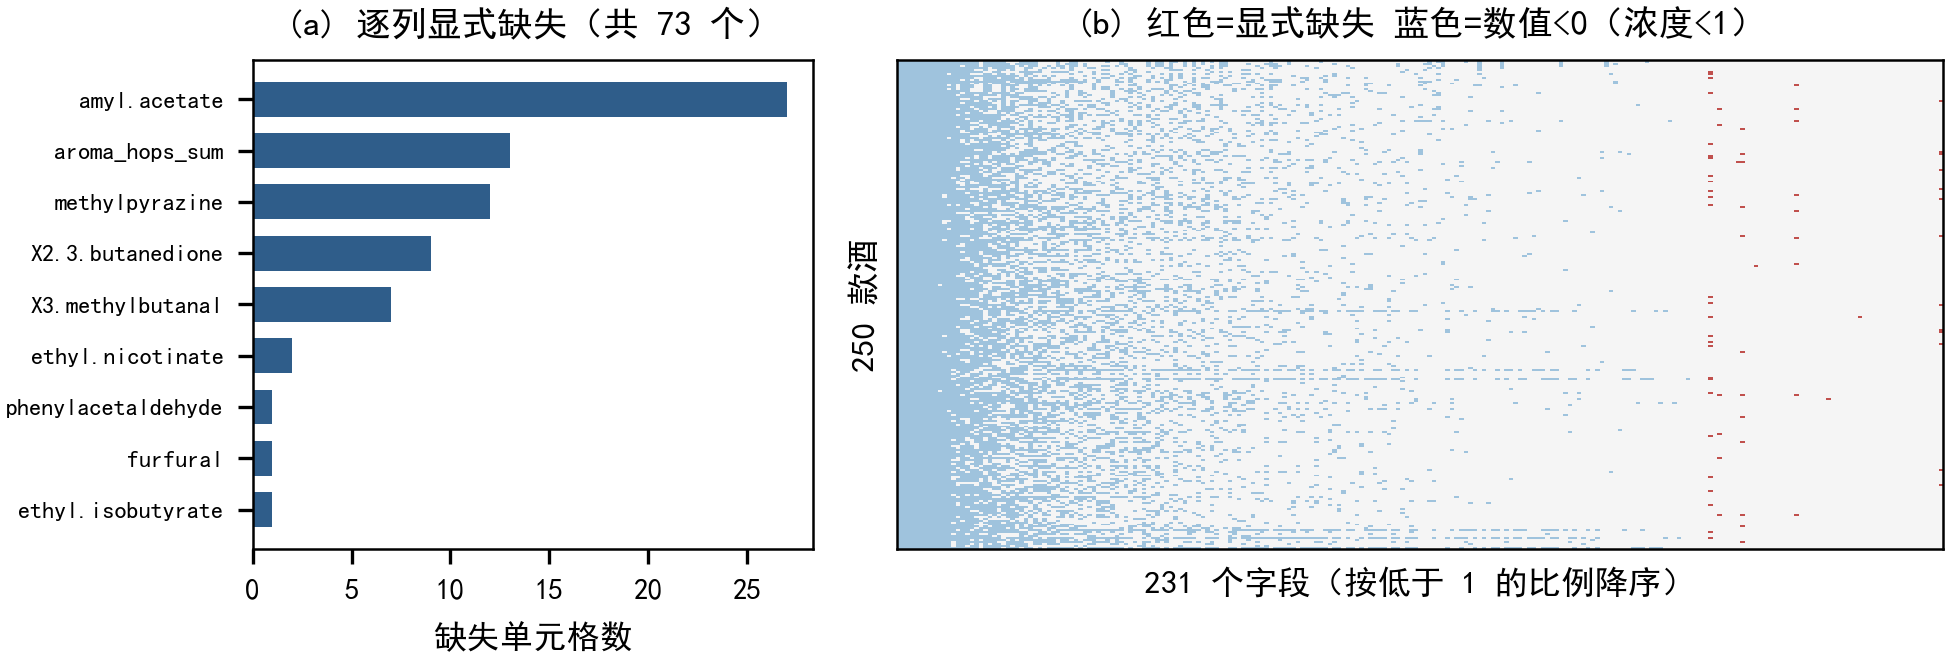
\includegraphics[width=0.98\textwidth]{figures/fig03_missing.png}
\caption{缺失与低值结构。(a) 231 个数值字段的显式缺失量，9 列有缺失，\texttt{amyl.acetate} 最多 27 格；(b) $250\times231$ 矩阵中缺失与负值的空间分布，缺失呈点状，负值呈面状。}
\label{fig:missing}
\end{figure*}

图\ref{fig:missing}(a) 显示显式缺失的列分布，(b) 显示 $250\times231$ 矩阵中缺失与负值的空间分布：缺失是点状，负值是面状。真正影响建模的是低值密集和评分端点的覆盖不足，而不是 73 个显式缺失；4.csv 没有 NaN，但每款酒只有 3--14 名品评员，端点估计的不确定性随人数下降。显式缺失由训练折填补处理，低值密集需要在对数尺度上建模，评分端点的覆盖不足只能通过面板聚合和区间估计控制。

\subsection{评分端点重建}

4.csv 是标准化后的感官分值，不能直接当作 0--6 分标签；0--6 端点需由公开逐人评分重建。4.csv 为 $250\times53$，50 个目标列的均值为 $-0.063$～$0.063$、标准差为 0.37～0.86，符合中心化/标准化后的尺度，与 0--6 原始分不符。各列均值接近 0、标准差小于 1，说明 4.csv 是对原始 0--6 分做中心化/标准化后的结果；列间标准差不齐，说明标准化未统一到单位方差。该表用于样本对应、目标定义和标准化核查，不作为回归标签；它仍保留样本间的相对差异，可用于检查目标分布和异常酒样，但不能还原 0--6 分，也不能替代逐人评分。面板均分的取值范围仍是 0--6，而 4.csv 的标准化值可正可负，两者不能在同一损失函数下混用；4.csv 的列均值和标准差只能确认标准化，不能反推出原始 0--6 分的线性变换参数。

8.xlsx 的字段说明指向作者公开的逐人评分数据。据此重建的面板包含 16 名品评员，每款酒 3--14 人、中位 8 人，共 2197 条 0--6 评分。16 名品评员以匿名编号出现，每款酒的品评员集合不同；按 beer 编号与附件对齐后，30 个 Aroma/Flavour 属性分成两组核对，20 个共用项单独核对。面板人数不等意味着端点精度不等，直接比较不同酒的均分会把精度差异混入误差。2197 条评分是重建端点的全部原始信息；任何汇总都会损失一部分分布信息，故本文保留逐条评分用于分布端点。

记第 $b$ 款酒、第 $j$ 个属性、第 $t$ 名品评员的第 $r$ 次评分为 $s_{btrj}$，$T_b$ 为评过该酒的品评员集合，$n_{bt}$ 为同一人的重复次数。面板均分为
\begin{equation}\label{eq:panelmean}
\bar s_{bj}=\frac{1}{|T_b|}\sum_{t\in T_b}\frac{1}{n_{bt}}\sum_{r=1}^{n_{bt}}s_{btrj},
\end{equation}
七级分布为
\begin{equation}\label{eq:dist}
q_{bjk}=\frac{1}{|T_b|}\sum_{t\in T_b}\frac{1}{n_{bt}}\sum_{r=1}^{n_{bt}}\mathbf{1}\{s_{btrj}=k\},
\end{equation}
其中 $k=0,\ldots,6$。

分母 $|T_b|$ 是实际评过该酒的品评员数，不是全体 16 人；每款酒的端点只使用自己的面板，未评人员不按 0 分计入。式\eqref{eq:panelmean} 与式\eqref{eq:dist} 都先在人内对重复评分取平均，再在人之间等权平均。同一人对同一杯酒的重复评分高度相关，若按原始条目数加权，评分次数多的人会主导端点；等权处理则让每名品评员对一款酒只投一票。同一人可能对同一杯酒给出多次评分，$n_{bt}$ 可能大于 1；先平均再等权等价于把每人的重复评分压缩成一条观测。面板均分与七级分布共享同一套人员权重，因此二者的差异只来自汇总方式，不来自样本集合。

平方损失下均值最优，绝对损失下中位数最优，累计分布损失下完整分布最优，0--1 损失下众数最优。三种端点对应三种决策损失：面板均分对应平方损失，七级分布对应累计分布或 RPS 损失，众数 $\hat g_{bj}=\arg\max_k q_{bjk}$ 对应 0--1 精确等级损失。本文不把三者压成一个标签，而是在第一问分别报告均分误差、分布距离和众数一致率。3--4 人面板的端点不确定性明显大于 8 人以上面板，第一问按人数分组报告覆盖率和误差，避免把面板人数差异误判为模型差异；众数对人数少的面板更敏感，3--4 人时众数可能只反映一两个品评员的选择。

\subsection{维度映射与提交口径}

评分卡与 4.csv 的目标可按字典一一映射，但字段名和模板公式不能直接照搬。3.xlsx 含 12 个 beer\_* 评分卡和 1 个 summary，12 张评分卡对应 12 款示例酒，summary 汇总这些酒的目标列；评分卡只用于维度定义，不直接提供 250 款酒的得分。每张卡左栏 Aroma、右栏 Flavour，两栏各含 Malt、Hops、Esters 三组，每组 4 个描述词加 1 个组汇总；乙醛 1 项，口感 4 项，缺陷 6--7 项，另有香料与 Lambic 专项。映射结果见表\ref{tab:dims}：A/F 前缀各 15 项，共 30 项核心；其余 20 项为口感、缺陷、香料、酸味与总体。这 50 个目标列同时定义第一问的输出、第二问的响应变量和第三问的感官画像维度。

\begin{table*}[t]
\centering\small\renewcommand{\arraystretch}{1.15}
\caption{评分卡分组与 4.csv 目标的字典映射。A/F 前缀各 15 项，其余 20 项为共用目标；乙醛项没有独立目标列。}
\label{tab:dims}
\begin{tabular}{@{}>{\raggedright\arraybackslash}p{0.155\textwidth}>{\raggedright\arraybackslash}p{0.555\textwidth}>{\raggedright\arraybackslash}p{0.105\textwidth}>{\raggedright\arraybackslash}p{0.075\textwidth}@{}}
\toprule
评分卡分组（项数） & 4.csv 字段 & 归属 & 目标数 \\
\midrule
Malt（4 子项 + 1 汇总） & A\_malt\_all, A\_malt\_grain, A\_malt\_bread, A\_malt\_cara, A\_malt\_burn；F 侧同构 & A\_/F\_ & 10 \\
Hops（4 子项 + 1 汇总） & A\_hops\_all, A\_hops\_citrus, A\_hops\_tropical, A\_hops\_noble, A\_hops\_woody；F 侧同构 & A\_/F\_ & 10 \\
Esters（4 子项 + 1 汇总） & A\_esters\_all, A\_esters\_ethac, A\_esters\_isoaa, A\_esters\_flower, A\_esters\_fruity；F 侧同构 & A\_/F\_ & 10 \\
Acetaldehyde（1） & — & — & 0 \\
口感（4） & body, bitternes, co2, aftertaste & 共用 & 4 \\
缺陷（6--7） & dms, metallic, X4vg, diacetyl, t2n, stale\_hops, barnyard & 共用 & 7 \\
香料、酸味与总体（9） & acidity, sweetness, orange, coriander, clove, lactic, acetic, alcohol, overall & 共用 & 9 \\
\midrule
合计 & A 15 项、F 15 项、共用 20 项 & & 50 \\
\bottomrule
\end{tabular}
\end{table*}

4.csv 中 A\_malt\_*、A\_hops\_*、A\_esters\_* 各 5 项，F 侧同构；组汇总以 \_all 结尾，共 6 项，三组汇总分别为 A/F\_malt\_all、A/F\_hops\_all、A/F\_esters\_all，组汇总与 4 个描述词共同构成 5 项，不能只取子项而漏掉汇总。Aroma 栏可映射 15 项（3 组 $\times$ 5），Flavour 栏同理；口感 4 项、缺陷 7 项、香料与总体 9 项构成其余 20 项。乙醛 1 项在 4.csv 中没有独立目标列，故不进入 50 项目标。字段名差异来自评分卡模板与监督表的两次命名：A/F\_ester\_fruity 在 4.csv 中写作 A/F\_esters\_fruity，4vg 写作 X4vg；若按字符串直接匹配，这几个字段会丢失。本文按显式字典映射，字典以 4.csv 的 50 个列名为准，逐项记录评分卡组别、A/F 归属和是否汇总；映射表写入交付包的字段清单，预测时按列名而非列序取数，不依赖评分卡模板公式。bitternes 等拼写按原表保留，避免合并时产生重复列。

提交口径为 50 项全部建模并输出，核心 30 项单列；20 个其他项用于缺陷约束、风格画像和总体评价。核心 30 项是训练面板的主评分维度，20 个其他项多为缺陷或风格专项，两类项目的量纲和稀疏性不同，分开报告更便于按决策场景取用。评分卡的组别划分与 0--6 强度标度符合训练面板的感官评价流程\cite{schreurs2024}；但乙醛位置没有独立目标列，组汇总也不能按模板公式直接重算，直接套公式会把无监督项算进目标，因此本文以字段名和组别字典为准。预测输出按 50 列对齐 4.csv 的列序，核心 30 项与其余 20 项用同一套字段清单标记，便于下游按组取用；映射表同时作为训练、预测和评价三处的字段白名单，避免不同脚本各自解释列名。
